% !TEX encoding = UTF-8 Unicode
\documentclass[a4paper]{article}

\usepackage{color}
\usepackage{url}
\usepackage[T2A]{fontenc} % enable Cyrillic fonts
\usepackage[utf8]{inputenc} % make weird characters work
\usepackage{graphicx}
\usepackage{placeins}

\usepackage[english,serbian]{babel}
%\usepackage[english,serbianc]{babel} %ukljuciti babel sa ovim opcijama, umesto gornjim, ukoliko se koristi cirilica

\usepackage[unicode]{hyperref}
\hypersetup{colorlinks,citecolor=green,filecolor=green,linkcolor=blue,urlcolor=blue}

\usepackage{listings}

%\newtheorem{primer}{Пример}[section] %ćirilični primer
\newtheorem{primer}{Primer}[section]

\definecolor{mygreen}{rgb}{0,0.6,0}
\definecolor{mygray}{rgb}{0.5,0.5,0.5}
\definecolor{mymauve}{rgb}{0.58,0,0.82}

\lstset{ 
  backgroundcolor=\color{white},   % choose the background color; you must add \usepackage{color} or \usepackage{xcolor}; should come as last argument
  basicstyle=\scriptsize\ttfamily,        % the size of the fonts that are used for the code
  breakatwhitespace=false,         % sets if automatic breaks should only happen at whitespace
  breaklines=true,                 % sets automatic line breaking
  captionpos=b,                    % sets the caption-position to bottom
  commentstyle=\color{mygreen},    % comment style
  deletekeywords={...},            % if you want to delete keywords from the given language
  escapeinside={\%*}{*)},          % if you want to add LaTeX within your code
  extendedchars=true,              % lets you use non-ASCII characters; for 8-bits encodings only, does not work with UTF-8
  firstnumber=1000,                % start line enumeration with line 1000
  frame=single,	                   % adds a frame around the code
  keepspaces=true,                 % keeps spaces in text, useful for keeping indentation of code (possibly needs columns=flexible)
  keywordstyle=\color{blue},       % keyword style
  language=Python,                 % the language of the code
  morekeywords={*,...},            % if you want to add more keywords to the set
  numbers=left,                    % where to put the line-numbers; possible values are (none, left, right)
  numbersep=5pt,                   % how far the line-numbers are from the code
  numberstyle=\tiny\color{mygray}, % the style that is used for the line-numbers
  rulecolor=\color{black},         % if not set, the frame-color may be changed on line-breaks within not-black text (e.g. comments (green here))
  showspaces=false,                % show spaces everywhere adding particular underscores; it overrides 'showstringspaces'
  showstringspaces=false,          % underline spaces within strings only
  showtabs=false,                  % show tabs within strings adding particular underscores
  stepnumber=2,                    % the step between two line-numbers. If it's 1, each line will be numbered
  stringstyle=\color{mymauve},     % string literal style
  tabsize=2,	                   % sets default tabsize to 2 spaces
  title=\lstname                   % show the filename of files included with \lstinputlisting; also try caption instead of title
}

\begin{document}

\title{\vspace{-3.0cm}Na osnovu člana 20 zakona o autorskim i srodnim pravima ovaj naslov Vam nije dostupan\\
\large \vspace{0.5cm}Seminarski rad u okviru kursa\\Metodologija stručnog i naučnog rada\\ Matematički fakultet}

\author{Strahinja Mitrić, Nemanja Gružanić, Petar Perišić, Nikola Mandić\\ strahinjamitric123@gmail.com, nemanjagruzanic996@gmail.com,\\ petar-perisic@outlook.com, mandinikola@gmail.com
}

\maketitle
%\date{9.~april 2015.}
\abstract{Da li ste ikada preuzeli neku
muzičku numeru sa interneta? A film? 
Ukoliko jeste - vrlo je verovatno da ste prekršili nekoliko zakona.
Ovaj rad će Vam kroz veliki broj primera približiti pojam intelektualne svojine,
ko ima pravo na nju i kako se ona štiti. Dodatno, istražujemo pojmove poput patenta, autorskog
prava i poslovne tajne, kao i kako se ovi pojmovi sprovode u računarstvu. 
Takođe istražujemo kakav uticaj intelektualna svojina ima na ekonomiju i 
koje posledice možete snositi ukoliko ne poštujete ove zakone u Srbiji.
}

\tableofcontents

\newpage

\section{Uvod}
\label{sec:uvod}
\subsection{Intelektualna svojina}
Šta prvo pomislite kada čujete pesmu 'Ajs Ajs Bejbi' (engl. \emph{Ice Ice Baby}) američkog repera Vanile Ajs?
Pored toga što se zapitate zašto bi iko pustio ovu pesmu, primetićete da Vam je ova pesma već odnekud poznata.
To su takođe primetili Dejvid Bouvi i članovi grupe 'Kvin' (engl. \emph{Queen}).
Naime Vanila Ajs je za svoju pesmu 'Ajs Ajs Bejbi' preuzeo kompletnu bas liniju pesme 'Ander Prešr' (engl. \emph{Under Pressure}).

Kako je svima vrlo brzo bilo jasno da je reč o plagijatu, a Dejvid Bouvi i grupa 'Kvin' nisu dobili
zasluge za komponovanje pesme, ova stvar je završila pred sudom.

Vanila Ajs je tvrdio da su melodije potpuno različite jer je dodao hip-hop bit preko bas linije. \cite{rollingstone}

Da li je Vanila Ajs u pravu, da li su melodije zaista potpuno različite? Ovim slučajem uvodimo pojam intelektualne svojine.

Prema definiciji intelektualna svojina je jedinstven proizvod ljudskog uma koji ima komercijalnu vrednost. \cite{texasUniv}
Dakle, intelektualnom svojinom smatramo knjige, muziku, film, slike, izume, softver itd.

Kako je Majkl J. Kuin naveo u svojoj knjizi 'Etika informatičkog doba', \cite{ethics} važno je razlikovati 
intelektualnu svojinu i ono na čemu je ona nastala. Dakle, kako Kuin navodi u primeru, ukoliko pesnik
napiše pesmu, intelektualna svojina je sama pesma, a ne parče hartije na kome je ona napisana.
Takođe, Kuin u svojoj knjizi navodi teoriju engleskog filozofa Džona Loka (1632-1704) o pravu na imovinu,
koju koristi kako bi pokazao da intelektualnu svojinu ne možemo porediti sa materijalnom svojinom.

\subsection{Kako zaštititi intelektualnu svojinu?}
Da li stvaralac ima prirodno pravo na svoje delo? Ukoliko se podsetimo primera Vanile Ajsa, moramo
dobro razmisliti.

Ono što pravo na intelektualnu svojinu predstavlja je zapravo pravo na sopstvenu ideju. Dakle, ono što 
intelektualnu svojinu razlikuje od posedovanja objekata ili sličnog, jeste upravo to što intelektualnu
svojinu primarno odlikuju jedinstvenost i kreativnost.

Kako bi bolje razumeli pravo na intelektualnu svojinu, uveli pojam zaštite intelektualne svojine,
pozvaćemo se još jednom na knjigu Majkla J. Kuina, \cite{ethics} gde je naveo sledeći primer: \newline 
Kakva prava na svoja dela bi imao Vilijam Šekspir da ih je neko prepisao i objavio pre njega? U primeru se navodi
Šekspirovo delo 'Hamlet'. Dakle, kako delo nije ukradeno već prepisano, Šekspir ga još uvek poseduje, međutim
više ne može kontrolisati ko može pročitati delo. Šta više  kradljivac može izvoditi javne predstave
Hamleta i zarađivati novac na osnovu toga.

Iz primera uviđamo da je krađa intelektualne svojine dosta različita od krađe postojanih objekata.
Kako Kuin kaže 'Ukoliko ukrademo nečija kola, on ih više ne može voziti. Ali ukoliko ukrademo nečiju šalu, 
obadvoje je sada možemo ispričati'.

Na osnovu navedenog, samo nam se nameće pitanje kako zaštititi intelektualnu svojinu? Odgovor na to pitanje
dajemo u poglavlju \ref{subsec:autorska} gde bolje objašnjavamo zbog čega je Vanila Ajs morao da potpiše Dejvida Bouvija i grupu
Kvin kao koautore svog hita 'Ice Ice baby'. Ali pre toga osvrnimo se malo na istorijat.

%Još u doba stare Grčke Platon je sa ogorčenjem govorio kako ćemo se sve manje oslanjati na sopstveno pamćenje a sve više na spise i druge vrste očuvanja podataka. U svojoj knjizi 'Ethics for the information age', M. Quinn postavlja pitanje kakvo bi pravo Šekspir imao na svoja dela da se neko prisetio da ih prepiše i objavi pre njega?
%\newline
%Već kroz ova dva podatka možemo uočiti polaritet na koji će se ovaj rad fokusirati i koji predstavlja suštinu problematike intelektualne svojine danas, a to je da tehnologija olakšava pristup informacijama što se, pojednostavljeno rečeno, protivi očuvanju intelektualne svojine, tačnije nedodirljive imovine koja je rezultat kreativnosti, među koju spadaju izumi, imena, simboli, slike, kompozicije i tako dalje. 

\section{Istorijat}
Monopolski statut (1624) smatra se početkom zaštite patentnog, a Anin statut (1710) početkom zaštite autorskih prava. Ova dva statuta, oba nastala u Britaniji, zajedno nam daju čvrste početke koncepta intelektualne svojine. Naime oba su doneta sa idejom zaštite stvaralaca od kraljevskih poreza jer je kruna shvatila da isti često koče napredak obećavajućih biznisa. Prvobitno korišćeni termin bio je pisana svojina a intelektualna svojina kao takva prvi put se pominje 1769. godine, dok se primer savremene upotrebe prvi put može uočiti tek 1808. 

Današnja svetska organizacija za intelektualnu svojinu nastala je tek 1967. godine, nasledivši dotadašnji ujedinjeni međunarodni biro za zaštitu intelektualne svojine koji datira još od 1893. kao sjedinjenje sekretarijata Pariske (1883) i Bernske (1886) konvencije.

\section{Prava intelektualne svojine}	
\label{sec:prava_int_svoj}

Prava intelektualne svojine uključuju patente, autorska prava, prava industrijskog dizajna, zaštitne znakove, prava na varijacije biljaka, ambalaže, geografske indikacije i u nekim nadležnostima poslovne tajne. Intelektualna svojina je definisana
teritorijalnim zakonima ali pored toga postoje standardi minimalnih zahteva za
svaku državu mada se gotovo po pravilu snažnije sprovode u razvijenijim
zemljama što manje razvijene zemlje često koriste kao razlog za verovanje da im
se ograničava pristup tehnologijama i brzoj globalizaciji. Savremeno očuvanje
intelektualne svojine ne radi savršeno kako možemo videti na primeru 'YouTube'-a
koji konstantno pokušava da obriše i demonetizuje video snimke koji ne poštuju
prava intelektualne svojine, ali usled ogromnog saobraćaja i korišćenja veštačke inteligencije u navedene svrhe, često greši te biva optužen za cenzuru.

\subsection{Patenti}
\label{subsec:patenti}

Patent je način na koji vlada daje izumitelju eksluzivno pravo na deo intelektualne svojine. Patent je sasvim drugačiji od poslovne tajne jer je patent javni dokument koji daje detaljan opis pronalaska. Vlasnik patenta može sprečiti druge da naprave, koriste ili prodaju izum za vreme trajanja patenta. Trenutno vreme trajanja patenta je 20 godina.

Dr. Edvin Lend je izmislio "instant"\space fotografiju. Kompanija koju je osnovao, Polaroid Corporation, imala je 10 patenata koji štite pronalzak filma koji se razvijao u roku od 60 sekundi. Polaroid nije licencirao ove patente drugim firmama. Kada je Kodak 1976. godine predstavio svoju "instant" kameru, Polaroid je to iskoristio za pokretanje tužbe. 1985. godine sud je odlučio da je Kodak prekršio sedam od deset Polaroidovih patenata. Šest godina kasnije Kodak je platio Polaroidu svotu od 925 miliona dolara.

\subsection{Autorska prava}
\label{subsec:autorska}

Autorsko pravo u određenom vremenskom periodu štiti od neautorizovanog kopiranja ili adaptiranja umetničkih, pisanih, fotografskih i na druge načine predstavljanja Vaše ideje. Ono ne štiti samu ideju, ali u nekim slučajevima - na primer kompjuterski kôd - može biti najefikasniji način da zaštitite Vašu intelektualnu svojinu.
Dakle, u slučaju pesme 'Ice Ice Baby', Vanila Ajs je neautorizovano kopirao i adaptirao 
bas liniju pesme 'Under Pressure'. Pošto je pesma bila pod autorskim pravima Dejvida Bouvija i
grupe 'Kvin', na kraju sudskog spora morao je da ih potpise kao koautore svog najveceg hita.
Autorsko pravo proističe automatski nastankom autorskog dela i ne zahteva troškove. To je važno zato što lako može da se ustanovi datum porekla ideje ili njene izmene. Međutim, ne pruža Vam se zaštita od nekog ko nezavisno dođe do iste ili slične ideje. Konkurent može reći da je njegova ideja slučajno slična Vašoj ili da je Vaša ideja kopija njegove. Kako možete dokazati da je Vaša ideja original?

Sledeći koraci Vam mogu pomoći da dokažete da ste nosilac autorskih prava u kasnijem sporu.

\begin{itemize}
\item[$-$] Pravite pisane opise, crteže, fotografije itd. Štampajte Vaše ideje ili ih režite na CD ili DVD.
\item[$-$] Stavite Vaše dokumente ili disk u sigurno zalepljenu kovertu na kojoj se nalazi potpisana i datirana izjava nezavisnog svedoka, koja svedoči da je koverta zapečaćena onog datuma kada ju je on ili ona pregledao.
\item[$-$] Pošaljite kovertu preporučenom poštom samom sebi ili mestu za sigurno čuvanje i čuvajte poštansku potvrdu s jasnim datumom.
\item[$-$] Koverta mora ostati neotvorena dok to ne zahteva sud. (Savetuje se da imate više od jedne koverte za slučaj da se Vaš zahtev za autorskim pravom proverava više nego jednom. Otvoreni koverat više nije validan kao dokaz autorskog prava).
\end{itemize}

\subsection{Prava industrijskog dizajna}
\label{subsec:dizajn}

Pravo industrijskog dizajna je pravo na intelektualnu svojinu koje štiti dizajn objekata koji nisu čisto praktične prirode. Industrijski dizajn sastoji se od stvaranja oblika, osobina ili kompozicija obrazaca ili boja, ili kombinacije obrazaca i boja u tri dimenzionoj formi zarad isticanja estetske vrednosti. U Evropskoj uniji poznatiji je kao dizajn zajednice.

\subsection{Zaštitni znakovi}
\label{subsec:trademark}

Zaštitni znak ili žig (\emph{engl. Trademark}) je reč, simbol, slika, zvuk ili boja koju kompanija koristi za identifikaciju robe. Dodeljivanjem žiga nekom proizvodu, vlada kompaniji daje pravo da ga koristi i pravo da spreči druge komapnije da ga koriste. Koristeći zaštitni znak kompanija može steći ime brenda. Društvo ima koristi od brendiranja jer brendiranje omogućava potrošačima da imaju više poverenja u kvalitet proizvoda koji kupuju. 

Kada je kompanija prva koja plasira prepoznatljiv proizvod, postoji rizik da će njegovo ime postati uobičajena imenica koja se koristi za opisivanje bilo kog sličnog proizvoda. Primer nekih robnih marki su: "yo yo", "aspirin", "termos" \space i "grudnjak".

\subsection{Prava na varijacije biljaka}
\label{subsec:granje}

Usled kalemljenja i genetske modifikacije naučnici često stvaraju nove vrste biljaka. Ukoliko se pokaže da se one dovoljno razlikuju od prethodnih i da nisu već otkrivene, datim naučnicima se može dati pravo intelektualne svojine nad datom varijacijom.

\newpage

\subsection{Geografske indikacije}
\label{subsec:geo}

Naznaka da proizvod dolazi iz određenog predela koji se diči visokim kvalitetom izrade takvih proizvoda može potpasti pod intelektualnu svojinu. Primeri su Klekovača iz Bajine Bašte, Newcastle Brown Ale, pomorandže sa Floride, Vina Novoga Sveta, Futoški kupus, grčki Feta sir.

\subsection{Poslovne tajne}
\label{subsec:poslovne}

Poslovna tajna je poverljiv deo intelektualne svojine koji kompaniji pruža prednost na tržištu. Primeri poslovnih tajni uključuju formule, procese, vlasničke dizajne, strateške planove, liste klijenata i druge informacije. Pravo kompanije da zaštiti svoje poslovne tajne široko su priznate od strane vlada širom sveta. Kompanije moraju preduzeti aktivne mere kako bi sprečile da njihova poslovna tajna bude otkrivena. Na primer, zaposleni koji imaju pristup poslovnoj tajni, morali su potpisati neki vid sporazuma o poverljivosti. Poslovna tajna koja je među najpoznatijima je i formula za Coca-Cola sirup. Formula se nalazi unutar jednog sefa u Atlanti, SAD. Samo nekoliko ljudi u kompaniji zna celu formulu, ali su potpisali sporazum o tajnosti. Zadatak izrade sirupa je podeljen između različitih grupa zaposlenih. Svaka grupa pravi samo deo konačne smese, tako da niko u ovim grupama ne zna ceo recept.

Prednost poslovnih tajni je što one nikada ne ističu. Coca-Cola čuva svoju tajnu već više od 100 godina.
Vrednost poslovnih tajni je u njihovoj poverljivosti. Zbog toga poslovne tajne nisu dobar način da se zaštite mnogi oblici intelektualne svojine. Na primer, nema smisla za kompaniju da napravi film koji će se čuvati kao poslovna tajna, jer kompanija profitira od filma ako dopusti da se taj film gleda, što ga ne čini više poverljivim.

Primer gde je moguće da dođe do 'curenja' informacija je prilikom odabranog zapošljavanja radnika u nekoj kompaniji. Firma može zahtevati od zaposlenih da potpišu ugovore o poverljivosti, ali ne može izbrisati pamćenje radnika koji u nekom trenutku krene raditi za konkurentsku firmu.

\section{Primena u računarstvu}
\label{primena_u_racuarstvu}

Kao što smo već ranije napomenuli, pod pojmom intelektualne svojine spada i softver.
Softver čine računarski programi i prateći podaci koji određuju izračunavanja koje vrši
računar. \cite{p1} Kada je u pitanju softver, zaštita intelektualne svojine se sprovodi putem
softverskih licenci.
Softverska licenca je pravni dokument kojim je regulisano korišćenje i
distribucija softvera. Takođe, omogućava krajnjem korisniku dozvolu da koristi jednu ili
više kopija nekog softvera na takav način da štiti sva prava autora. Pre nego što detaljnije
opišemo softverske licence, osvrnimo se na sam softver.

Grubo govoreći, softver možemo podeliti na vlasnički softver (engl. proprietary software)
i nevlasnički softver. Vlasnički softver je softver čiji je vlasnik pojedinac ili kompanija
(obično neko ko je softver razvio), postoje oštra ograničenja za njegovo korišćenje i,
gotovo isključivo, njegov izvorni kod čuva se u tajnosti.

Nevlasnički softver možemo podeliti na sledeći način:
    \begin{description}
        \item[$\bullet$] Šerver softver (engl. shareware software)
        \item[$\bullet$] Friver softver (engl. freeware software)
        \item[$\bullet$] Javni softver (engl. public software)
        \item[$\bullet$] Softver otvorenog koda (engl. open source software) ili besplatan softver (engl. free software) 
    \end{description}
Ono što odlikuje nevlasnički softver je da se distribuira besplatno, ili u retkim slučajevima šerver 
softvera po niskim cenama. \cite{free_philosophy}

Softver otvorenog koda je softver kojem se besplatno može pristupiti, koristiti, modifikovati i deliti
(u originalnoj ili izmenjenoj formi) od strane bilo koga. Softver otvorenog koda je obično pisan od strane velikog
broja autora i distribuira se pod odgovarajućom licencom. Licence za otvoreni kod se oslanjaju na autorska
prava. \cite{free_philosophy}

\subsection{Vlasnički softver}
\label{vlasnicki_softver}

Kod vlasničkog softvera, primarna svrha softverske licence je da ograniči
upotrebu softvera u skladu sa 
poslovnom strategijom vlasnika prava. Kao posledica toga, vlasničke licence su često veoma restriktivne za 
kranje korisnike. One obično dozvoljavaju korišćenje softvera samo za njegovu navedenu svrhu, na samo jednom
računaru, pri čemu zabranjuju korisnicima da kopiraju, redistribuiraju ili menjaju rad i izričito zabranjuju
stvaranje derivata koristeći delove softvera.
Kao što smo već napomenuli, kod vlasničkog softvera se čuva u tajnosti pa prema tome programi pod 
vlasničkim licencama se obično distribuiraju isključivo samo u binarnom obliku i zabranjuju ispitivanje
programskog koda ili obrnutog inžinjeringa bilo kog dela programa.

Većina vlasničkog softvera je zaštićena autorskim pravima na softver. Na osnovu autorskih prava na softver,
proizvođač softvera zadržava sva prava na algoritme i karakteristike softvera, dok se izvorni kod (engl. Source code)
tretira kao poslovna tajna. Proizvođač softvera određuje specifične uslove koršćenja softvera u ugovoru o licenci 
krajnjeg korisnika (engl. End-user license agreement). Na primer, kako bi korisnik koristio muzički servis Ajtjuns (engl. iTunes),
korisnik ne sme koristiti dati softver za dizajn, konstrukciju ili distribuciju nuklearnog ili hemijskog oružja. \cite{apple}

\subsection{Softver otvorenog koda}
\label{softver_otvorenog_koda}

Ko kontroliše Vaš računar? Da li ga kontrolišete Vi ili neka kompanija čiji softver koristite? Grubo govoreći računar izvršava
programe a programi se sastoje od naredbi. Dakle računar će izvršiti bilo koju naredbu koju želite. Kako je programski kod 
vlasničkog softvera poslovna tajna, postavljeno pitanje uopšte nije besmisleno.

Isto pitanje veoma često postavlja i Ričard Stolman, jedan od začetnika pokreta slobodnog i otvorenog softvera 
(engl. free/open-source software movement). Slobodan i otvoren softver predstavlja fundamentalno drugačiji 
pristup licenciranju softvera.

Osnovna namera softvera otvorenog koda je da se maksimizira otvorenost koda i prava korisnika a da
se minimiziraju prepreke za korišćenje softvera. Upravo ovakav pristup softveru podstiče kopileft (engl. Copyleft).
Kopileft je strategija korišćenja zakona o autorskim pravima, o kom smo već govorili u \ref{subsec:autorska}, u cilju 
ostvarivanja politike podsticanja jednakog prava na kopiranje, deljenje, modifikovanje i poboljšavanje autorskih dela. \cite{copyleft}
Ovakav pristup softveru, kao autorskom delu, podstiče veliki broj licenci koje nam upravo to omogućavaju.
Neke od najčešće korišćenih licenci softvera otvorenog koda su GNU General Public License (GPL), Apache License,
Creative Commons Licenses, MIT License, BSD License, itd. Svaka od navedenih licenci varira na neke važne načine, ali sve nam daju 
slobodan, otvoren i nedeskriminatorski pristup softveru. 
U tabeli \ref{tab:tabela1} su prikazane detaljnije razlike između licenci otvorenog koda. 
Nedeskriminatorski pristup softveru znači da nijednoj
kategoriji korisnika ili distributera ne sme biti zabranjena upotreba softvera. \cite{opensource}
Posledica ovog pristupa je da softver otvorenog koda može biti korišćen i u komercijalne svrhe, što se često i događa.

Jedna od glavnih prednosti softvera otvorenog koda je upravo ta što je izvorni kod javno dostupan. \cite{opensource} Prednost ovog pristupa je 
što na izvornom kodu programa može raditi veliki broj programera, što podstiče saradnju i pojednostavljuje kontinuinalni 
razvoj programa. Takođe, jedna od ključnih posledica je naravno da možete biti da Vaš računar radi ono što i želite da radi. 

U današnje vreme, često se dešava da vlasnički softver prikuplja razne podatke o svojim korisnicima,
hteli oni to ili ne. Na primer, često se govori o kompanijama poput Gugl (engl. Google) i Majkrosoft (engl. Microsoft) 
kako špijuniraju svoje korisnike. Ovo je jedna od važnijih razlika između vlasničkog softvera i softvera otvorenog koda.

\begin{table}[h!]
    \begin{center}
        \caption{ Detaljnije razlike između softverskih licenci. }
        \begin{tabular}{|c|c|c|c|c|} \hline
            \emph{Licenca} & \emph{Korišćenje} & \emph{Distribucija} & \emph{Patent} & \emph{Modifikacija} \\ \hline
            GNU GPLv3 & Da & Kopileft & Da & Kopileft\\ \hline
            Academic Free License & Da & Da & Da & da \\ \hline
            Mozilla Public License & Da & Kopileft & Da & Kopileft \\ \hline
            BSD License & Da & Da & Da & Da \\ \hline
            Apache License & Da & Da & Da & Da  \\ \hline
            Creative Commons Zero & Da & Da & Ne & Da \\ \hline
            MIT license & Da & Da & Ne & Da \\ \hline
            Microsoft Public License & Da & Da & Ne & Da \\ \hline
            Eclipse Public License & Da & Ograničeno & Da & Ograničeno \\ \hline
        \end{tabular}
        \label{tab:tabela1}
    \end{center}
\end{table}

\section{Ciljevi zakona intelektualne svojine}

\subsection{Finansijski podsticaj}
\label{subsec:fin}

Osnovna motivacija zaštite intelektualne svojine bila je i ostaje zaštita inovatora
i njegovog otkrića od okoline - države sa svojim porezima ili drugih
inovatora ili ljudi koji žele da profitiraju tuđim kreativnim radom.
Ova zaštita takođe ima za cilj da motiviše inovatore da nastave sa svojim
radom pruživši im ekskluzivno pravo da zarade od svog izuma. Radovi poput \cite{patents} 
pokazuju da opstanak firme direktno zavisi od broja patenata koje ona napravi.
S druge strane, rad \cite{patents} pokazuje nam da pored zaštite intelektualne svojine 
postoje i drugi načini motivisanja i zaštite inovatora poput nagrađivanja, 
ugovora fiksne cene i aukcija, ali takođe pokazuje kako je, dobro
organizovana, zaštita intelektualne svojine najbolje od ovih rešenja. Slika~\ref{fig:ComDesign} nam pokazuje sve veći porast iskorišćenosti prava na zaštitu intelektualne svojine u svetu.

\newpage

\begin{figure}
\begin{center}
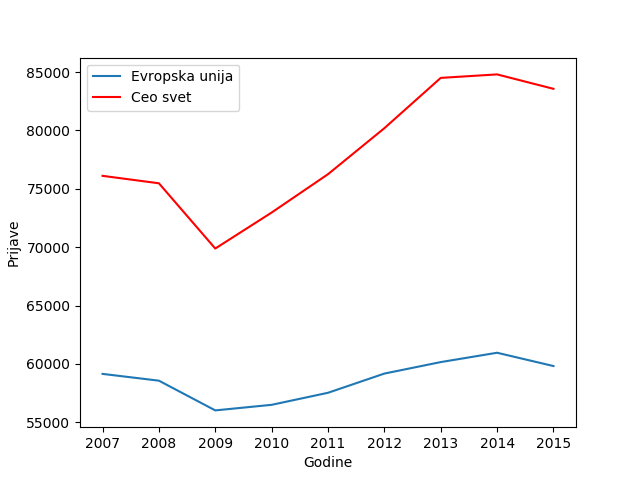
\includegraphics[scale=0.4615]{eu_vs_cs.png}
\end{center}
\caption{Prikaz broja prijava dizajna zajednice (engl. community design) po godinama u svetu i EU.}
\label{fig:ComDesign}
\end{figure}

\subsection{Ekonomski rast}
\label{subsec:ekon}

Različite ekonomije mogu iznedriti različite modele zaštite intelektualne
svojine i pokazuje se da je mnogo bolje imati diverzitet u tome jer nijedan
model ne može važiti za sve države ni za sve ekonomije. Na grafiku \ref{fig:pat_gdp} možemo videti korelaciju između bruto domaćeg proizvoda zemalja i jačine zakona kojim one čuvaju intelektualnu svojinu svojih građana.

\begin{figure}
\begin{center}
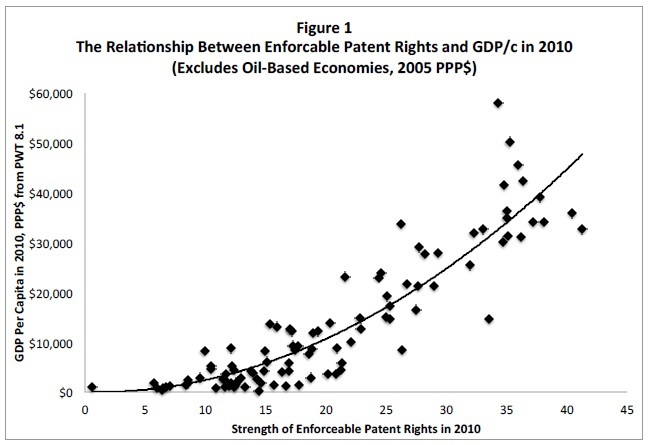
\includegraphics[scale=0.4615]{patents_and_gdp.jpg}
\end{center}
\caption{Veza između striktnosti očuvanja patenata zemalja i njihovog bruto domaćeg proizvoda.}
\label{fig:pat_gdp}
\end{figure}

\newpage

\section{Sprovođenje u Srbiji}

U sistemu državne uprave Republike Srbije postoji Zavod za intelektualnu svojinu u čijoj su nadležnosti poslovi koji se odnose na prava industrijske svojine, autorsko i srodna prava.

Sprovođenje prava intelektualne svojine podrazumeva primenu delotvornih i srazmernih administrativnih, građanskih mera i kazni od strane nadležnih organa protiv onih koji su uključeni u krivotvorenje i pirateriju u cilju stvaranja jednakih uslova poslovanja za nosioce prava.

Svako neovlašćeno korišćenje predmeta prava intelektualne svojine predstavlja povredu prava intelektualne svojine. Nadležni organi za sprovođenje prava intelektualne svojine u Srbiji dele se na administrativne (ministarstva finansija, unutrašnjih poslova, poljoprivrede, trgovine, šumarstva i ostali) i sudsko-tužilačke (sudovi i tužilaštva).

\subsection{Kazne}

U vezi sa prvim po redu krivičnim delom, krivični zakon \cite{KZ} je u članu 198. propisao da svako ko pod svojim imenom ili imenom drugog, u celini ili delimično objavi, stavi u promet primerke tuđeg autorskog dela ili interpretacije, ili na drugi način javno saopšti tuđe autorsko delo ili interpretaciju, kazniće se novčanom kaznom ili zatvorom do tri godine. U istom članu stoji i da je svaka izmena ili prerada tuđeg autorskog dela ili tuđe snimljene interpretacije, bez dozvole autora, odnosno interpretatora kažnjiva novčanom kaznom ili kaznom zatvora do jedne godine. Zatim, stavljanje u promet primeraka tuđeg autorskog dela ili interpretacije na način kojim se vređa čast ili ugled autora ili izvođača, kazniće se novčanom kaznom ili zatvorom do šest meseci.

Naredno krivično delo, neovlašćeno iskorišćavanje autorskog dela ili predmeta srodnog prava, sadržano je u članu 199. Ono postoji ukoliko neko neovlašćeno objavi, snimi, umnoži, ili na drugi način javno saopšti u celini ili delimično autorsko delo, interpretaciju, fonogram, videogram, emisiju, računarski program ili bazu podataka. Sankcija za ovo delo je kazna zatvora do tri godine. Identična kazna propisana je i za učinioca koji stavi u promet ili sa namerom stavljanja u promet drži neovlašćeno umnožene ili neovlašćeno stavljene u promet primerke autorskog dela ili predmeta srodnog prava (interpretaciju, fonogram, videogram itd.). Ako je navedene radnje učinilac krivičnog dela preduzeo u nameri pribavljanja imovinske koristi za sebe ili drugog, tj. u lukrativne svrhe, kazniće se zatvorom od šest meseci do pet godina.

Treće krivično delo, iz grupe krivilnih dela protiv intelektualne svojine, jeste neovlašćeno uklanjanje ili menjanje elektronske informacije o autorskom i srodnim pravima. Svako ko neovlašćeno ukloni ili izmeni elektronsku informaciju o autorskom ili srodnom pravu, ili stavi u promet, uveze, izveze, emituje ili na drugi način javno saopšti zaštićeni sadržaj sa kojeg je elektronska informacija o pravima neovlašćeno uklonjena ili izmenjena kazniće se kumulativno novčanom kaznom i zatvorom do tri godine. Kod ovog krivičnog dela, ne postoje ’’izvedena’’ ili ’’modifikovana’’ krivična dela, kao kod prethodna dva. Predmeti iz ovog krivičnog dela će se oduzeti i uništiti.

Što se tiče, povrede pronalazačkog prava (koje predstavlja jednu od celina industrijske svojine), propisana je novčana kazna ili kazna zatvora do tri godine za onoga ko neovlašćeno proizvodi, uvozi, izvozi, nudi radi stavljanja u promet, stavlja u promet, skladišti ili koristi u privrednom prometu proizvod ili postupak zaštićen patentom. Ako je ovim delom pribavljena imovinska korist ili prouzrokovana šteta drugome u iznosu koji prelazi milion dinara, učiniocu je zaprećena kazna zatvora od jedne do osam godina. Dakle, najteža kazna koja je propisana za krivična dela iz ove grupe. U okviru ovog člana, predviđeno je i još da neovlašćeno objavljivanje ili činjenje dostupnim suštine tuđeg prijavljenog pronalaska, pre nego što je on objavljen na zakonom utvrđeni način, predstavlja krivično delo sa sankcijom za učinioca u vidu novčane kazne ili zatvora do dve godine. Pored toga, ko još i neovlašćeno podnese patentnu prijavu ili u prijavi ne navede ili lažno navede pronalazača, kazniće se zatvorom od šest meseci do pet godina. Predmeti koji su proistekli iz dela neovlašćene proizvodnje, uvoza, izvoza, stavljanja u promet itd. i usled kojih je učinilac pribavio imovinsku korist ili prouzrokovao štetu, oduzeće se i uništiti.

Na kraju, za neovlašćeno korišćenje tuđeg dizajna (koje predstavlja pravo u okviru pronalazačkog prava), zaprećena je novčana kazna ili zatvor do tri godine. Jedna od ove dve kazne će se primeniti ako učinilac na svom proizvodu koji se nalazi u prometu, neovlašćeno upotrebi, u celosti ili delimično, tuđi prijavljeni, odnosno zaštićeni dizajn proizvoda. Pored toga, kazniće se i onaj ko neovlašćeno objavi ili na drugi način učini dostupnim javnosti predmet prijave tuđeg dizajna pre nego što je on objavljen na zakonom propisani način, novčanom kaznom ili kaznom zatvora do jedne godine. Proizašli proizvodi će se oduzeti, što je identično sa krivičnim delom povrede moralnih prava autora i interpretatora.

%dodati izvore koriscene na http://nomcentarngo.com/krivicna-dela-protiv-intelektualne-svojine/#_ftnref1

\label{sec:srb}

\section{Zaključak}
\label{sec:zakljucak}

Intelektualna svojina predstavlja jedan od bitnijih aspekata bavljenja naukom, računarstvom ili bilo kojom stvaralačkom granom i omogućava nam da svoja dela zaštitimo i time pomognemo kako sebi tako i ekonomskoj sredini u kojoj se nalazimo. U poslednjih nekoliko decenija zasnovani su mnogi zakoni i regulative koji nam ovo omogućavaju, ali isto tako porastao je i broj posledica koje nas mogu sačekati ukoliko ove pogodnosti ne iskoristimo. Zajednice koje nam obezbeđuju mogućnost da svoja dela štitimo svesne su kolektivne dobiti koju to nosi, a na nama kao individuama ostaje da te pogodnosti iskoristimo i postaramo se da naša dela ne budu iskorišćena u svrhu dolaženja do protivpravne materijalne koristi drugih lica. Ovim radom opisali smo vrste intelektualne svojine i uslove koje one moraju ispuniti, dali smo kratak istorijat i motivaciju za uspostavljanje ovog pojma i objasnili kako se primenjuje u računarstvu i u našoj zemlji. Nadamo se da smo čitaoce motivisali da čuvaju i poštuju kako svoju, tako i tuđu intelektualnu svojinu i da smo ih dovoljno dobro uputili u načine na koje to mogu činiti.

\addcontentsline{toc}{section}{Literatura}
\appendix
\bibliography{seminarski} 
\bibliographystyle{plain}

\end{document}
